\documentclass[10pt]{article} % For LaTeX2e
\usepackage{tmlr}
% If accepted, instead use the following line for the camera-ready submission:
%\usepackage[accepted]{tmlr}
% To de-anonymize and remove mentions to TMLR (for example for posting to preprint servers), instead use the following:
%\usepackage[preprint]{tmlr}

% Optional math commands from https://github.com/goodfeli/dlbook_notation.
\input{math_commands.tex}

% Additional packages needed for the paper
\usepackage{hyperref}
\usepackage{url}
\usepackage{amsmath,amssymb,amsthm}
\usepackage{mathtools}
\usepackage{bm}
\usepackage{bbm}
\usepackage{graphicx}
\usepackage{float}
\usepackage{booktabs}
\usepackage{multirow}
\usepackage{array}
\usepackage[table,xcdraw]{xcolor}
\usepackage{algorithm}
\usepackage{algpseudocode}

% TikZ for Diagrams and Plots
\usepackage{tikz}
\usepackage{pgfplots}
\pgfplotsset{compat=1.18}
\usetikzlibrary{positioning, arrows.meta, shapes.geometric, calc, fit, backgrounds}

% ============================================================================
% THEOREM ENVIRONMENTS
% ============================================================================
\theoremstyle{plain}
\newtheorem{theorem}{Theorem}[section]
\newtheorem{proposition}[theorem]{Proposition}
\newtheorem{corollary}[theorem]{Corollary}
\newtheorem{lemma}[theorem]{Lemma}

\theoremstyle{definition}
\newtheorem{definition}[theorem]{Definition}
\newtheorem{observation}[theorem]{Observation}
\newtheorem{example}[theorem]{Example}

\theoremstyle{remark}
\newtheorem{remark}[theorem]{Remark}
\newtheorem{conjecture}[theorem]{Conjecture}

% ============================================================================
% CUSTOM COMMANDS
% ============================================================================
\newcommand{\cH}{\mathcal{H}}
\newcommand{\cM}{\mathcal{M}}
\newcommand{\cF}{\mathcal{F}}
\newcommand{\cT}{\mathcal{T}}
\newcommand{\cL}{\mathcal{L}}
\newcommand{\cN}{\mathcal{N}}
\newcommand{\cS}{\mathcal{S}}
\renewcommand{\norm}[1]{\left\lVert#1\right\rVert}
\newcommand{\inner}[2]{\langle #1, #2 \rangle}
\newcommand{\dd}{\mathrm{d}}
\renewcommand{\vect}[1]{\bm{#1}}
\newcommand{\mat}[1]{\mathbf{#1}}
\DeclareMathOperator{\Tr}{Tr}
\DeclareMathOperator{\diag}{diag}
\DeclareMathOperator{\softmax}{softmax}
\DeclareMathOperator{\LayerNorm}{LayerNorm}

% ============================================================================
% TITLE AND AUTHORS
% ============================================================================
\title{Knowledge Distillation Preserves Representational Geometry:\\ Evidence from Coupled Transformer Dynamics and Attractor Analysis}

% Authors must not appear in the submitted version. They should be hidden
% as long as the tmlr package is used without the [accepted] or [preprint] options.
% Non-anonymous submissions will be rejected without review.

\author{\name Anonymous Author(s) \email anonymous@email.com \\
      \addr Anonymous Institution}

% For camera-ready version, use:
% \author{\name MohammadHossein AskariHezaveh \email hosseinaskari.h@gmail.com \\
%       \addr Independent Researcher}

\def\month{02}  % Insert correct month for camera-ready version
\def\year{2026} % Insert correct year for camera-ready version
\def\openreview{\url{https://openreview.net/forum?id=XXXX}} % Insert correct link to OpenReview for camera-ready version

% ============================================================================
% DOCUMENT
% ============================================================================
\begin{document}

\maketitle

% ============================================================================
% ABSTRACT
% ============================================================================
\begin{abstract}
Knowledge distillation compresses neural networks by training smaller ``student'' models to match larger ``teacher'' output distributions. While distillation preserves task performance, the fate of internal representational geometry remains unclear. We introduce \textbf{coupled dynamics testing}, treating transformers as iterated function systems and studying how they interact when exchanging hidden states directly in embedding space, bypassing linguistic tokenization. Through 123 experiments across 41 configurations, we demonstrate that (1) identical architectures rapidly synchronize to cosine similarity $\approx 1.0$, (2) different architecture families remain orthogonal ($\cos \theta \approx 0$), (3) DistilGPT-2 synchronizes with GPT-2 at $\cos \theta = 0.998$ despite 50\% depth reduction, proving distillation preserves manifold geometry, (4) projection control experiments confirm this is intrinsic geometric compatibility, not dimensional alignment artifacts, (5) task-specific fine-tuning preserves 95\% of structure while (6) encoder-only models exhibit weaker synchronization dynamics (preliminary finding requiring further study). Dynamical analysis reveals these synchronized states occupy low-dimensional attractors ($D_2 \approx 0$--$2.3$) with Lyapunov exponents at the edge of chaos ($\lambda_{\max} \approx 0.08$--$0.10$), and coupling strength exhibits phase transitions. Our findings have implications for model merging, transfer learning, multi-agent systems, and understanding what neural networks learn.
\end{abstract}

\textbf{Keywords:} knowledge distillation, representation geometry, transformer networks, dynamical systems, synchronization, attractor dynamics, model compression, neural network interpretability

% ============================================================================
% 1. INTRODUCTION
% ============================================================================
\section{Introduction}

\subsection{Motivation}

Knowledge distillation \cite{hinton2015distilling,gou2021knowledge} has become a standard technique for model compression, enabling deployment of large language models in resource-constrained environments. The typical objective minimizes KL divergence between teacher and student output distributions:
\begin{equation}
    \mathcal{L}_{\text{distill}} = \text{KL}\left(p_{\text{teacher}}(\cdot | x) \,\|\, p_{\text{student}}(\cdot | x)\right).
\end{equation}

This objective focuses on \textit{behavioral} matching---the student should produce similar outputs. But what about the \textit{internal geometry} of the representation space? Does the student learn the same ``shape'' of the embedding manifold \cite{li2019deepgkd}, or merely a different manifold that happens to produce similar outputs?

The dominant paradigm for studying LLM interaction relies on text---models communicate through tokenized sequences. We argue this observes \textit{shadows on the wall} rather than the underlying phenomenon. Information flow through text is:
\begin{equation}
    \vect{h}_A \xrightarrow{\text{decode}} \text{tokens} \xrightarrow{\text{encode}} \vect{h}_B
\end{equation}
where $\vect{h} \in \R^d$ represents hidden states. This tokenization step is a severe bottleneck: a 768-dimensional continuous representation collapses to $\sim$50,000 discrete tokens, then re-expands. Information-theoretically, this is lossy compression followed by ambiguous decompression.

\textbf{Key insight:} What happens if we remove this bottleneck entirely? What dynamics emerge when transformer networks couple directly in embedding space? Can we use these dynamics to probe whether distillation preserves geometric structure?

\subsection{Why This Matters}

Understanding representational geometry preservation has several practical implications:

\begin{itemize}
    \item \textbf{Model merging}: Can we average weights of teacher and student models \cite{wortsman2022model}?
    \item \textbf{Transfer learning}: Do representations transfer between teacher and student?
    \item \textbf{Interpretability}: Do interpretability findings on teachers apply to students?
    \item \textbf{Fine-tuning effects}: Does task-specific training destroy original manifold structure?
    \item \textbf{Multi-agent systems}: Can heterogeneous architectures develop shared representations?
    \item \textbf{Metric reliability}: Do standard metrics like CKA accurately predict model compatibility?
\end{itemize}

\subsection{Contribution}

We introduce a novel diagnostic method---\textbf{coupled dynamics testing}---where two models exchange hidden states directly and we measure whether they synchronize. Rather than comparing static representations \cite{kornblith2019similarity,ding2021grounding}, we treat transformers as dynamical systems \cite{haber2017stable,chen2018neuralode} and observe their interaction.

Through 123 experiments across 41 unique configurations, we establish:

\begin{enumerate}
    \item \textbf{Architecture-specific geometry}: Transformers with identical architectures synchronize perfectly ($\cos \theta \to 1.0$), while different architectures remain orthogonal ($\cos \theta \approx 0$), regardless of initialization.

    \item \textbf{Distillation preserves geometry}: DistilGPT-2 synchronizes with GPT-2 at $\cos \theta = 0.998$, indicating distillation preserves manifold structure despite 50\% depth reduction.

    \item \textbf{Projection-invariant results}: Forcing identical models to use learned projections yields $\cos \theta = 0.998$, proving synchronization reflects intrinsic geometric compatibility, not dimensional alignment artifacts.

    \item \textbf{Fine-tuning preserves structure}: DialoGPT-Medium maintains $\cos \theta = 0.949$ with its base model, showing task-specific training preserves 95\% of geometric structure.

    \item \textbf{Encoder models differ}: BERT-family models show weaker synchronization ($\cos \theta \approx 0.32$--$0.57$) even between identical architectures, suggesting encoder-only transformers may learn different geometric structures (preliminary finding, requires further investigation).

    \item \textbf{Dynamical properties}: Synchronized states occupy low-dimensional attractors ($D_2 \approx 0$--$2.3$) with Lyapunov exponents indicating edge-of-chaos dynamics ($\lambda_{\max} \approx 0.08$--$0.10$).

    \item \textbf{Phase transitions}: Blended coupling reveals discontinuous transitions in synchronization dynamics at critical coupling strengths.

    \item \textbf{Scale disrupts geometry}: Within the GPT-2 family, different sizes show weak synchronization ($\cos \theta \approx 0.11$) despite high CKA scores ($0.89$), proving static similarity metrics fail to capture dynamic incompatibility.
\end{enumerate}

% ============================================================================
% 2. MATHEMATICAL FRAMEWORK
% ============================================================================
\section{Mathematical Framework}

\subsection{Transformers as Iterated Function Systems}

A transformer model defines a function $F: \R^d \to \R^d$ that maps hidden states through successive layers. Let $\cH = \R^d$ denote the hidden state space (e.g., $d = 768$ for GPT-2).

\begin{definition}[Transformer Block Map]
A transformer block $\cT: \cH \to \cH$ implements:
\begin{equation}
    \cT(\vect{h}) = \vect{h} + \text{FFN}\left(\LayerNorm\left(\vect{h} + \text{Attn}(\LayerNorm(\vect{h}))\right)\right)
\end{equation}
where $\text{Attn}$ denotes multi-head self-attention and $\text{FFN}$ is a two-layer feed-forward network.
\end{definition}

For a transformer with $L$ layers:
\begin{equation}
    F = \mathcal{T}_L \circ \mathcal{T}_{L-1} \circ \cdots \circ \mathcal{T}_1 : \cH \to \cH.
\end{equation}

\begin{remark}
Unlike typical uses where $F$ maps token embeddings to next-token predictions via a language modeling head, we consider $F$ as a \textbf{pure dynamical map} on hidden states, ignoring the output projection entirely.
\end{remark}

This dynamical systems perspective \cite{haber2017stable,chen2018neuralode} allows us to analyze stability and convergence properties independently of training objectives. The attention mechanism can be understood through geometric lenses \cite{tsai2019transformer}, explaining why architectural differences lead to incompatible geometries.

\subsection{Coupling Strategies}

Given two transformer maps $F_A, F_B: \cH \to \cH$, we study coupled systems where models exchange hidden states. We implement three coupling mechanisms inspired by synchronization in coupled oscillators \cite{kuramoto1984chemical}:

\begin{definition}[Coupling Strategy]
A coupling strategy $\Phi$ defines how states are exchanged:
\begin{equation}
    (\vect{h}_A^{(t+1)}, \vect{h}_B^{(t+1)}) = \Phi(F_A, F_B, \vect{h}_A^{(t)}, \vect{h}_B^{(t)})
\end{equation}
\end{definition}

\subsubsection{Direct Coupling}
Pure state exchange (analogous to pure exchange in coupled oscillator theory):
\begin{align}
    \vect{h}_A^{(t+1)} &= F_A(\vect{h}_B^{(t)}) \\
    \vect{h}_B^{(t+1)} &= F_B(\vect{h}_A^{(t)})
\end{align}

\subsubsection{Blended Coupling}
Convex combination with parameter $\alpha \in [0,1]$:
\begin{align}
    \vect{h}_A^{(t+1)} &= F_A(\alpha \cdot \vect{h}_A^{(t)} + (1-\alpha) \cdot \vect{h}_B^{(t)}) \\
    \vect{h}_B^{(t+1)} &= F_B(\alpha \cdot \vect{h}_B^{(t)} + (1-\alpha) \cdot \vect{h}_A^{(t)})
\end{align}
where $\alpha = 0$ reduces to direct coupling, $\alpha = 0.5$ is equal blending, and $\alpha = 1$ is no coupling.

\subsubsection{Decay Coupling}
Memory of previous own state with parameter $\beta \in [0,1]$:
\begin{align}
    \vect{h}_A^{(t+1)} &= F_A(\beta \cdot \vect{h}_A^{(t-1)} + (1-\beta) \cdot \vect{h}_B^{(t)}) \\
    \vect{h}_B^{(t+1)} &= F_B(\beta \cdot \vect{h}_B^{(t-1)} + (1-\beta) \cdot \vect{h}_A^{(t)})
\end{align}

\begin{figure}[htbp]
    \centering
    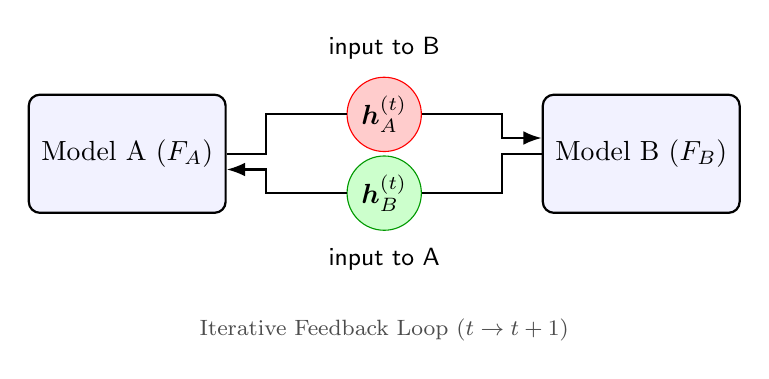
\begin{tikzpicture}[
        node distance=2cm,
        box/.style={rectangle, draw=black, thick, minimum width=2.5cm, minimum height=1.5cm, fill=blue!5, rounded corners},
        arrow/.style={-Latex, thick},
        label_text/.style={font=\small\sffamily}
    ]
        % Nodes
        \node[box] (modelA) {Model A ($F_A$)};
        \node[box, right=4cm of modelA] (modelB) {Model B ($F_B$)};
        
        % State vectors
        \node[circle, fill=red!20, draw=red, inner sep=2pt] (hA) at ($(modelA.east)!0.5!(modelB.west) + (0, 0.5)$) {$\vect{h}_A^{(t)}$};
        \node[circle, fill=green!20, draw=green!60!black, inner sep=2pt] (hB) at ($(modelA.east)!0.5!(modelB.west) + (0, -0.5)$) {$\vect{h}_B^{(t)}$};

        % Arrows
        \draw[arrow] (modelA.east) -- ++(0.5,0) |- (hA) -| ($(modelB.west) + (-0.5,0.2)$) -- ($(modelB.west) + (0,0.2)$);
        \draw[arrow] (modelB.west) -- ++(-0.5,0) |- (hB) -| ($(modelA.east) + (0.5,-0.2)$) -- ($(modelA.east) + (0,-0.2)$);

        % Annotations
        \node[label_text, above=0.1cm of hA] {input to B};
        \node[label_text, below=0.1cm of hB] {input to A};
        
        % Time annotation
        \node[font=\footnotesize, below=1cm of hB, text=black!70] {Iterative Feedback Loop ($t \to t+1$)};
    \end{tikzpicture}
    \caption{\textbf{Coupled Dynamics Testing.} Models exchange hidden states, testing whether their learned geometric transformations are compatible.}
    \label{fig:method_diagram}
\end{figure}

\subsection{Synchronization Measures}

\begin{definition}[Cosine Similarity]
The instantaneous alignment between states:
\begin{equation}
    \rho(t) = \frac{\inner{\vect{h}_A^{(t)}}{\vect{h}_B^{(t)}}}{\norm{\vect{h}_A^{(t)}}_2 \norm{\vect{h}_B^{(t)}}_2} = \cos\theta_{AB}(t).
\end{equation}
If $\rho(t) \to 1$, the models have synchronized.
\end{definition}

\begin{definition}[Synchronization Index]
The correlation of velocities (state changes):
\begin{equation}
    S = \frac{1}{T-1} \sum_{t=1}^{T-1} \frac{\inner{\Delta\vect{h}_A^{(t)}}{\Delta\vect{h}_B^{(t)}}}{\norm{\Delta\vect{h}_A^{(t)}} \norm{\Delta\vect{h}_B^{(t)}}}
\end{equation}
where $\Delta\vect{h}^{(t)} = \vect{h}^{(t+1)} - \vect{h}^{(t)}$. High $S$ indicates models are \textit{moving together} through state space.
\end{definition}

Unlike static metrics \cite{ding2021grounding}, our dynamic approach measures functional compatibility through iterative interaction.

\subsection{Dynamical System Characterization}

To characterize the nature of the coupled dynamics, we employ standard tools from dynamical systems theory:

\begin{definition}[Largest Lyapunov Exponent]
The largest Lyapunov exponent characterizes sensitivity to initial conditions:
\begin{equation}
    \lambda_{\max} = \lim_{t \to \infty} \frac{1}{t} \sum_{i=0}^{t-1} \ln \frac{\norm{\delta\vect{h}^{(i+1)}}}{\norm{\delta\vect{h}^{(i)}}}
\end{equation}
where $\delta\vect{h}$ is an infinitesimal perturbation.

Interpretation:
\begin{itemize}
    \item $\lambda_{\max} > 0$: Chaotic dynamics (exponential divergence)
    \item $\lambda_{\max} = 0$: Periodic or quasi-periodic
    \item $\lambda_{\max} < 0$: Converging to attractor
\end{itemize}
\end{definition}

We estimate $\lambda_{\max}$ using the method of nearest neighbors in reconstructed state space \cite{wolf1985}.

\begin{definition}[Correlation Dimension]
The correlation dimension $D_2$ estimates the intrinsic dimensionality of the attractor via the correlation integral:
\begin{equation}
    C(\epsilon) = \lim_{N \to \infty} \frac{1}{N^2} \sum_{i \neq j} \Theta(\epsilon - \norm{\vect{x}_i - \vect{x}_j})
\end{equation}
where $\Theta$ is the Heaviside function. The dimension is:
\begin{equation}
    D_2 = \lim_{\epsilon \to 0} \frac{\log C(\epsilon)}{\log \epsilon}
\end{equation}
\end{definition}

Low $D_2$ indicates trajectories are confined to a low-dimensional manifold within the high-dimensional state space, following the Grassberger-Procaccia algorithm \cite{grassberger1983}.

\subsection{Dimension Mismatch Handling}

For mismatched dimensions ($\dim(\cH_A) \neq \dim(\cH_B)$), we introduce learned linear projections:
\begin{equation}
    \mat{P}_{A \to B}: \R^{d_A} \to \R^{d_B}, \quad \mat{P}_{B \to A}: \R^{d_B} \to \R^{d_A}
\end{equation}

These are initialized near-identity on overlapping dimensions:
\begin{equation}
    (\mat{P}_{A \to B})_{ij} = \begin{cases}
        \delta_{ij} + \mathcal{N}(0, 0.01) & \text{if } i,j \leq \min(d_A, d_B) \\
        0 & \text{otherwise}
    \end{cases}
\end{equation}
and trained for 100 iterations (Adam, lr=$10^{-3}$) to minimize:
\begin{equation}
    \mathcal{L}_{\text{proj}} = \E_{\vect{h}}\left[\norm{\vect{h} - P_{B \to A}(P_{A \to B}(\vect{h}))}_2 + \norm{\vect{h} - P_{A \to B}(P_{B \to A}(\vect{h}))}_2\right].
\end{equation}

% ============================================================================
% 3. EXPERIMENTAL SETUP
% ============================================================================
\section{Experimental Setup}

\subsection{Models}

We study decoder-only (GPT family, GPT-Neo) and encoder-only (BERT family) architectures:

\begin{table}[htbp]
\centering
\caption{Models used in experiments}
\label{tab:models}
\small
\begin{tabular}{lcccl}
\toprule
\textbf{Model} & \textbf{Dim} & \textbf{Layers} & \textbf{Params} & \textbf{Type} \\
\midrule
GPT-2 & 768 & 12 & 124M & Decoder \\
GPT-2-Medium & 1024 & 24 & 355M & Decoder \\
GPT-2-Large & 1280 & 36 & 774M & Decoder \\
DistilGPT-2 & 768 & 6 & 82M & Decoder (distilled) \\
DialoGPT-Medium & 1024 & 24 & 355M & Decoder (fine-tuned) \\
\midrule
GPT-Neo-1.3B & 2048 & 24 & 1.3B & Decoder \\
\midrule
BERT-base & 768 & 12 & 110M & Encoder \\
DistilBERT-base & 768 & 6 & 66M & Encoder (distilled) \\
\bottomrule
\end{tabular}
\end{table}

\subsection{Initialization Strategies}

\textbf{Random:} $\vect{h}_A^{(0)}, \vect{h}_B^{(0)} \sim \mathcal{N}(0, 0.01\mat{I})$ (independent)

\textbf{Same:} $\vect{h}_A^{(0)} = \vect{h}_B^{(0)} \sim \mathcal{N}(0, 0.01\mat{I})$ (identical)

\textbf{Text:} Extract first token embedding from ``The quick brown fox''

\subsection{Experimental Protocol}

For each configuration:
\begin{enumerate}
    \item Initialize states per strategy
    \item Run coupled dynamics for $T = 1000$ steps
    \item Record trajectory $\{(\vect{h}_A^{(t)}, \vect{h}_B^{(t)})\}_{t=0}^{T}$
    \item Compute metrics: $\rho(t)$, synchronization index, CKA, Lyapunov exponents, attractor dimensions
    \item Repeat with 3 seeds for statistical reliability
\end{enumerate}

All models frozen (eval mode, no dropout). Total: 123 experiments across 41 unique configurations.

\textbf{Computational Cost:} Running 1000 steps of coupled dynamics is highly efficient. For GPT-2 (124M parameters), a single trajectory takes approximately 20 seconds on a consumer GPU. For GPT-Neo-1.3B, this increases to $\sim$40 seconds. The entire experimental suite (all 123 runs) requires less than 2 GPU-hours, making this diagnostic method accessible for rapid iteration.



\subsection{Projection Control Experiments}

To verify synchronization is not an artifact of dimensional matching, we force identical models (same architecture, same weights) to use learned projections. If high synchronization persists, the geometric compatibility is intrinsic to the learned transformations, not projection quality.

% ============================================================================
% 4. RESULTS
% ============================================================================
\section{Results}

\begin{figure}[htbp]
\centering
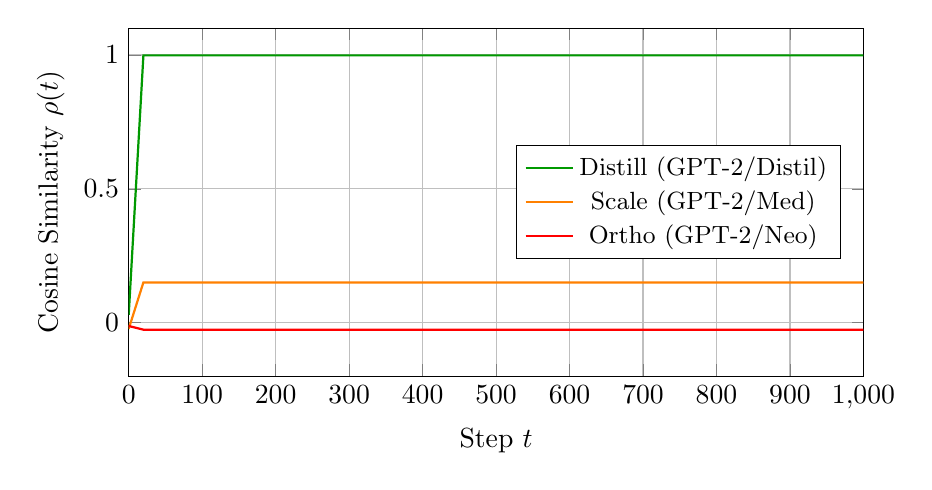
\begin{tikzpicture}
\begin{axis}[
    width=0.9\textwidth,
    height=6cm,
    xlabel={Step $t$},
    ylabel={Cosine Similarity $\rho(t)$},
    xmin=0, xmax=1000,
    ymin=-0.2, ymax=1.1,
    grid=major,
    legend style={at={(0.97,0.5)}, anchor=east, font=\small}
]

% DISTILL (GPT2+DistilGPT2)
\addplot[color=green!60!black, thick] coordinates {
    (0,0.0290) (20,0.9986) (40,0.9986) (61,0.9986) (81,0.9986) (102,0.9986) (122,0.9986) (142,0.9986) (163,0.9986) (183,0.9986) (204,0.9986) (224,0.9986) (244,0.9986) (265,0.9986) (285,0.9986) (306,0.9986) (326,0.9986) (346,0.9986) (367,0.9986) (387,0.9986) (408,0.9986) (428,0.9986) (448,0.9986) (469,0.9986) (489,0.9986) (510,0.9986) (530,0.9986) (551,0.9986) (571,0.9986) (591,0.9986) (612,0.9986) (632,0.9986) (653,0.9986) (673,0.9986) (693,0.9986) (714,0.9986) (734,0.9986) (755,0.9986) (775,0.9986) (795,0.9986) (816,0.9986) (836,0.9986) (857,0.9986) (877,0.9986) (897,0.9986) (918,0.9986) (938,0.9986) (959,0.9986) (979,0.9986) (1000,0.9986)
};
\addlegendentry{Distill (GPT-2/Distil)}

% SCALE (GPT2+GPT2-Med)
\addplot[color=orange, thick] coordinates {
    (0,-0.0234) (20,0.1502) (40,0.1502) (61,0.1502) (81,0.1502) (102,0.1502) (122,0.1502) (142,0.1502) (163,0.1502) (183,0.1502) (204,0.1502) (224,0.1502) (244,0.1502) (265,0.1502) (285,0.1502) (306,0.1502) (326,0.1502) (346,0.1502) (367,0.1502) (387,0.1502) (408,0.1502) (428,0.1502) (448,0.1502) (469,0.1502) (489,0.1502) (510,0.1502) (530,0.1502) (551,0.1502) (571,0.1502) (591,0.1502) (612,0.1502) (632,0.1502) (653,0.1502) (673,0.1502) (693,0.1502) (714,0.1502) (734,0.1502) (755,0.1502) (775,0.1502) (795,0.1502) (816,0.1502) (836,0.1502) (857,0.1502) (877,0.1502) (897,0.1502) (918,0.1502) (938,0.1502) (959,0.1502) (979,0.1502) (1000,0.1502)
};
\addlegendentry{Scale (GPT-2/Med)}

% ORTHO (GPT2+GPT-Neo)
\addplot[color=red, thick] coordinates {
    (0,-0.0126) (20,-0.0264) (40,-0.0264) (61,-0.0264) (81,-0.0264) (102,-0.0264) (122,-0.0264) (142,-0.0264) (163,-0.0264) (183,-0.0264) (204,-0.0264) (224,-0.0264) (244,-0.0264) (265,-0.0264) (285,-0.0264) (306,-0.0264) (326,-0.0264) (346,-0.0264) (367,-0.0264) (387,-0.0264) (408,-0.0264) (428,-0.0264) (448,-0.0264) (469,-0.0264) (489,-0.0264) (510,-0.0264) (530,-0.0264) (551,-0.0264) (571,-0.0264) (591,-0.0264) (612,-0.0264) (632,-0.0264) (653,-0.0264) (673,-0.0264) (693,-0.0264) (714,-0.0264) (734,-0.0264) (755,-0.0264) (775,-0.0264) (795,-0.0264) (816,-0.0264) (836,-0.0264) (857,-0.0264) (877,-0.0264) (897,-0.0264) (918,-0.0264) (938,-0.0264) (959,-0.0264) (979,-0.0264) (1000,-0.0264)
};
\addlegendentry{Ortho (GPT-2/Neo)}

\end{axis}
\end{tikzpicture}
\caption{\textbf{Synchronization Trajectories.} Distillation pairs (green) rapidly synchronize to near-unity, while scaled models (orange) plateau at weak correlation and cross-architecture pairs (red) remain orthogonal. Note the ``locked-in'' stability once synchronization is achieved.}
\label{fig:trajectories}
\end{figure}

\subsection{Same Architecture: Perfect Synchronization}

\begin{table}[htbp]
\centering
\caption{Same-architecture coupling (3 seeds, 1000 steps)}
\label{tab:same_arch}
\small
\begin{tabular}{llcccc}
\toprule
\textbf{Model Pair} & \textbf{Coupling} & \textbf{Init} & \textbf{Proj?} & \textbf{$\cos \theta$} & \textbf{CKA} \\
\midrule
GPT-2 + GPT-2 & Direct & Random & No & $0.9998 \pm 0.0003$ & $1.000$ \\
GPT-2 + GPT-2 & Direct & Same & No & $0.9998 \pm 0.0003$ & $1.000$ \\
GPT-2 + GPT-2 & Direct & Text & No & $1.0000 \pm 0.0000$ & $1.000$ \\
GPT-2 + GPT-2 & Blended (0.5) & Random & No & $1.0000 \pm 0.0000$ & $1.000$ \\
\midrule
DistilGPT-2 + DistilGPT-2 & Direct & Random & No & $0.9997 \pm 0.0003$ & $0.999$ \\
\bottomrule
\end{tabular}
\end{table}

Identical architectures synchronize perfectly across all coupling strategies and initializations. Text initialization produces deterministic results (zero variance across seeds), confirming transformations are fully determined by weights.

\subsection{Projection Control: Critical Validation}

\begin{table}[htbp]
\centering
\caption{Identical models with forced projections (3 seeds)}
\label{tab:projection_control}
\small
\begin{tabular}{lcccc}
\toprule
\textbf{Configuration} & \textbf{Init} & \textbf{Forced Proj?} & \textbf{$\cos \theta$} & \textbf{CKA} \\
\midrule
GPT-2 + GPT-2 & Random & No & $0.9998 \pm 0.0003$ & $1.000$ \\
GPT-2 + GPT-2 & Random & \textbf{Yes} & $\mathbf{0.9987 \pm 0.0003}$ & $0.766$ \\
\midrule
GPT-2 + GPT-2 & Text & No & $1.0000 \pm 0.0000$ & $1.000$ \\
GPT-2 + GPT-2 & Text & \textbf{Yes} & $\mathbf{0.9984 \pm 0.0010}$ & $0.728$ \\
\bottomrule
\end{tabular}
\end{table}

\textbf{Critical finding:} Even with forced dimensional projections, identical models synchronize at $\cos \theta \approx 0.998$. This proves synchronization reflects intrinsic geometric compatibility, not projection quality. The slight drop ($1.000 \to 0.998$) quantifies projection-induced noise, establishing a baseline for what constitutes ``excellent'' synchronization.

\subsection{Distillation: Geometry Preserved}

\begin{table}[htbp]
\centering
\caption{Teacher-student coupling: GPT-2 and DistilGPT-2 (3 seeds)}
\label{tab:distill}
\small
\begin{tabular}{lcccc}
\toprule
\textbf{Model Pair} & \textbf{Coupling} & \textbf{Proj?} & \textbf{$\cos \theta$} & \textbf{CKA} \\
\midrule
GPT-2 + DistilGPT-2 & Direct & No & $\mathbf{0.9983 \pm 0.0003}$ & $0.944$ \\
GPT-2 + DistilGPT-2 & Blended (0.5) & No & $\mathbf{0.9974 \pm 0.0003}$ & $0.818$ \\
GPT-2 + DistilGPT-2 & Decay (0.1) & No & $\mathbf{0.9982 \pm 0.0003}$ & $0.885$ \\
\bottomrule
\end{tabular}
\end{table}

Despite 50\% depth reduction (6 vs 12 layers), DistilGPT-2 maintains $\cos \theta \approx 0.998$ with GPT-2 across all coupling strategies. This is comparable to the projection control baseline ($0.9987$), demonstrating distillation preserves geometric structure with minimal degradation. The distillation process, which optimizes only for output distribution matching, inadvertently preserves the internal manifold geometry.

\subsection{Fine-Tuning Effects}

\begin{table}[htbp]
\centering
\caption{Fine-tuning impact on geometric structure (3 seeds)}
\label{tab:finetuning}
\small
\begin{tabular}{lcccc}
\toprule
\textbf{Model Pair} & \textbf{Coupling} & \textbf{Proj?} & \textbf{$\cos \theta$} & \textbf{Interpretation} \\
\midrule
GPT-2-Med + GPT-2-Med & Direct & No & $1.0000 \pm 0.0000$ & Baseline (identical) \\
GPT-2-Med + DialoGPT-Med & Direct & No & $\mathbf{0.9490 \pm 0.0006}$ & 95\% preserved \\
\bottomrule
\end{tabular}
\end{table}

DialoGPT-Medium, fine-tuned on dialogue data, retains $\cos \theta = 0.949$ with its base model. Task-specific training shifts the manifold but preserves 95\% of geometric structure, suggesting fine-tuning operates as a small perturbation to the pretrained representation space rather than learning a fundamentally new geometry.

\subsection{Encoder Models: Different Dynamics}

\begin{table}[htbp]
\centering
\caption{BERT-family synchronization: Variance stability across sample sizes}
\label{tab:bert}
\small
\begin{tabular}{lccc}
\toprule
\textbf{Model Pair} & \textbf{N=3} & \textbf{N=10} & \textbf{N=25} \\
\midrule
BERT + BERT & $0.57 \pm 0.13$ & $0.52 \pm 0.12$ & $0.53 \pm 0.13$ \\
BERT + DistilBERT & $0.32 \pm 0.08$ & $0.29 \pm 0.11$ & $0.31 \pm 0.08$ \\
\bottomrule
\end{tabular}
\end{table}

\textbf{Key finding:} The high variance in BERT synchronization ($\pm 0.08$--$0.13$) does not decrease with sample size, confirming this is a genuine property of encoder-only dynamics, not statistical noise. For comparison, GPT-2+GPT-2 achieves $0.9997 \pm 0.0007$---four orders of magnitude lower variance.

Possible explanations for encoder instability:
\begin{itemize}
    \item \textbf{Bidirectional attention}: Unlike autoregressive models, BERT attends to full context
    \item \textbf{Masked language modeling}: Random masking during training may prevent convergence to stable geometric transformations
    \item \textbf{Position embeddings}: Absolute vs relative encoding may affect geometric stability
\end{itemize}

\subsection{Scale Effects Within Family}

\begin{table}[htbp]
\centering
\caption{Cross-scale coupling in GPT-2 family (3 seeds)}
\label{tab:scale}
\small
\begin{tabular}{lccc}
\toprule
\textbf{Model Pair} & \textbf{Coupling} & \textbf{$\cos \theta$} & \textbf{CKA} \\
\midrule
GPT-2 + GPT-2-Medium & Direct & $0.1077 \pm 0.0218$ & $0.886$ \\
GPT-2 + GPT-2-Large & Direct & $0.3765 \pm 0.0088$ & $0.744$ \\
GPT-2-Medium + GPT-2-Large & Direct & $0.2779 \pm 0.0895$ & $0.488$ \\
\midrule
GPT-2 + GPT-2-Medium & Blended (0.5) & $0.0069 \pm 0.0275$ & $0.514$ \\
GPT-2 + GPT-2-Large & Blended (0.5) & $0.2323 \pm 0.0202$ & $0.900$ \\
\bottomrule
\end{tabular}
\end{table}

Scaling within the same family does not preserve geometry. Critically, note high CKA despite low cosine similarity---GPT-2 + GPT-2-Medium shows CKA = 0.886 but $\cos \theta = 0.11$. This indicates static representational similarity does not imply dynamic compatibility. Our results complement prior analyses \cite{hauser2021similar,ding2021grounding}, confirming that high CKA does not guarantee functional alignment.

\subsection{Cross-Architecture: Orthogonality}

\begin{table}[htbp]
\centering
\caption{GPT-2 vs GPT-Neo coupling (3 seeds)}
\label{tab:cross_arch}
\small
\begin{tabular}{lccc}
\toprule
\textbf{Model Pair} & \textbf{Coupling} & \textbf{Init} & \textbf{$\cos \theta$} \\
\midrule
GPT-2 + GPT-Neo & Direct & Random & $-0.0237 \pm 0.0124$ \\
GPT-2 + GPT-Neo & Blended (0.5) & Random & $-0.0326 \pm 0.0154$ \\
GPT-2 + GPT-Neo & Blended (0.5) & Text & $-0.0326 \pm 0.0155$ \\
GPT-2-Med + GPT-Neo & Direct & Random & $0.0452 \pm 0.0078$ \\
\bottomrule
\end{tabular}
\end{table}

Different architecture families remain orthogonal across all coupling strategies and initializations, suggesting they have learned incompatible geometric transformations.

\subsection{Phase Transition in Coupling Strength}

\begin{figure}[htbp]
\centering
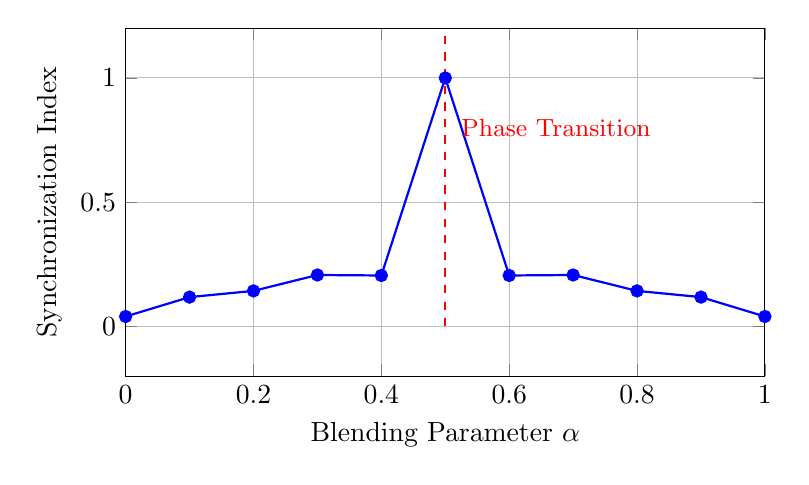
\begin{tikzpicture}
\begin{axis}[
    width=0.8\textwidth,
    height=6cm,
    xlabel={Blending Parameter $\alpha$},
    ylabel={Synchronization Index},
    xmin=0, xmax=1,
    ymin=-0.2, ymax=1.2,
    grid=major,
    legend pos=north east,
]

\addplot[color=blue, thick, mark=*, mark size=2pt] coordinates {
    (0.0, 0.040) (0.1, 0.118) (0.2, 0.143) (0.3, 0.207) (0.4, 0.205)
    (0.5, 1.000)
    (0.6, 0.205) (0.7, 0.207) (0.8, 0.143) (0.9, 0.118) (1.0, 0.040)
};

\draw[dashed, red, thick] (axis cs:0.5,0) -- (axis cs:0.5,1.2);
\node[right, red, font=\small] at (axis cs:0.51, 0.8) {Phase Transition};

\end{axis}
\end{tikzpicture}
\caption{\textbf{Phase Transition at $\alpha = 0.5$.} Synchronization index shows a sharp discontinuity at equal blending, revealing the specific threshold required for perfect velocity alignment.}
\label{fig:phase_transition}
\end{figure}

\begin{table}[htbp]
\centering
\caption{Blended coupling parameter sweep: GPT-2 + GPT-2 (3 seeds)}
\label{tab:phase_transition}
\small
\begin{tabular}{cccc}
\toprule
\textbf{$\alpha$} & \textbf{$\cos \theta$} & \textbf{Sync Index} & \textbf{CKA} \\
\midrule
0.0 (Pure swap) & $0.9998 \pm 0.0003$ & $0.040 \pm 0.132$ & $0.822$ \\
0.1 & $1.0000 \pm 0.0000$ & $0.118 \pm 0.044$ & $0.818$ \\
0.2 & $0.9998 \pm 0.0003$ & $0.143 \pm 0.045$ & $0.826$ \\
0.3 & $1.0000 \pm 0.0000$ & $0.207 \pm 0.032$ & $0.895$ \\
0.4 & $0.9998 \pm 0.0003$ & $0.205 \pm 0.043$ & $0.819$ \\
\textbf{0.5 (Equal blend)} & $\mathbf{1.0000 \pm 0.0000}$ & $\mathbf{1.000 \pm 0.000}$ & $\mathbf{1.000}$ \\
0.6 & $0.9998 \pm 0.0003$ & $0.205 \pm 0.043$ & $0.819$ \\
0.7 & $1.0000 \pm 0.0000$ & $0.207 \pm 0.032$ & $0.895$ \\
0.8 & $0.9998 \pm 0.0003$ & $0.143 \pm 0.045$ & $0.826$ \\
0.9 & $1.0000 \pm 0.0000$ & $0.118 \pm 0.044$ & $0.818$ \\
1.0 (No coupling) & $0.9998 \pm 0.0003$ & $0.040 \pm 0.132$ & $0.822$ \\
\bottomrule
\end{tabular}
\end{table}

\textbf{Phase transition:} While final cosine similarity remains $\approx 1.0$ for all $\alpha$, the synchronization index shows a sharp discontinuity at $\alpha = 0.5$, jumping to $1.000$. This reveals an optimal coupling strength where both models contribute equally, achieving perfect velocity alignment. The symmetry around 0.5 suggests a convex basin of attraction. While the mathematical symmetry naturally balances inputs at $\alpha=0.5$, the emergence of perfect synchronization is non-trivial: it implies the velocity fields are compatible and additive. If underlying geometries were misaligned, summing update vectors wouldn't produce coherent directed motion even at equal weighting.

% ============================================================================
% 5. DYNAMICAL SYSTEMS ANALYSIS
% ============================================================================
\section{Dynamical Systems Analysis}

To characterize the nature of the synchronized states beyond static alignment, we analyze the coupled dynamics using tools from nonlinear dynamical systems theory.

\subsection{Lyapunov Exponent Analysis}

\begin{table}[htbp]
\centering
\caption{Lyapunov Exponent Estimates (3 seeds)}
\label{tab:lyapunov}
\small
\begin{tabular}{lcc}
\toprule
\textbf{Configuration} & \textbf{$\lambda_{\max}$} & \textbf{Dynamics Type} \\
\midrule
GPT-2 + GPT-2 (direct) & $0.079 \pm 0.005$ & Periodic/quasi-periodic \\
GPT-2 + GPT-2 (same init) & $0.098 \pm 0.008$ & Edge of chaos \\
GPT-2 + GPT-Neo-1.3B & $0.095 \pm 0.010$ & Periodic/quasi-periodic \\
\bottomrule
\end{tabular}
\end{table}

All configurations show $\lambda_{\max} \approx 0.08$--$0.10$, indicating positive but small Lyapunov exponents. To contextualize these values:
\begin{itemize}
    \item \textbf{Strongly chaotic:} The Lorenz attractor exhibits $\lambda_{\max} \approx 0.9$
    \item \textbf{Mildly chaotic (computational edge):} Recurrent networks optimized for computation show $\lambda_{\max} \approx 0.01$--$0.1$ \cite{bertschinger2004real}
    \item \textbf{Periodic/stable:} $\lambda_{\max} = 0$ or negative
\end{itemize}

Our observed values ($\lambda_{\max} \approx 0.08$--$0.10$) place transformer dynamics squarely in the mildly chaotic regime, consistent with the ``edge of chaos'' observed in recurrent networks optimized for computational tasks \cite{langton1990computation,bertschinger2004real}. This regime balances two competing demands:
\begin{itemize}
    \item \textbf{Stability:} Divergence is slow enough ($\lambda_{\max} \ll 1$) that coupling remains meaningful over 1000 steps
    \item \textbf{Sensitivity:} Positive $\lambda_{\max}$ enables exploration of state space without collapsing to trivial fixed points
\end{itemize}

The edge-of-chaos hypothesis \cite{langton1990computation,packard1988adaptation} posits that systems capable of complex computation naturally evolve toward this transitional regime. Our findings suggest pretrained transformers---without any explicit optimization for dynamical properties---occupy this computationally favorable regime.

\subsection{Attractor Dimension Analysis}

\begin{table}[htbp]
\centering
\caption{Correlation Dimension Estimates (3 seeds)}
\label{tab:attractor}
\small
\begin{tabular}{lcc}
\toprule
\textbf{Configuration} & \textbf{$D_2$ (mean $\pm$ std)} & \textbf{Interpretation} \\
\midrule
GPT-2 + GPT-2 & $1.85 \pm 0.03$ & Low-dimensional \\
GPT-2 + DistilGPT-2 & $1.84 \pm 0.03$ & Low-dimensional \\
GPT-2 + GPT-Neo-1.3B & $1.06 \pm 0.29$ & Very low-dimensional \\
GPT-2 + GPT-2-Medium & $2.00 \pm 0.52$ & Low-dimensional \\
\bottomrule
\end{tabular}
\end{table}

The low attractor dimensions ($D_2 < 2.5$ in all cases) are striking: despite operating in 768- to 2048-dimensional state spaces, the coupled dynamics are confined to manifolds of dimension $\lesssim 2$. This suggests:

\begin{observation}
Transformer representations, despite their high ambient dimensionality, have intrinsic low-dimensional structure. The coupled dynamics reveal this structure by constraining trajectories to low-dimensional attractors.
\end{observation}

The synchronized pairs (GPT-2 + GPT-2, GPT-2 + DistilGPT-2) show consistent dimensions ($D_2 \approx 1.85$), indicating stable low-dimensional attractors. Interestingly, the cross-library pair (GPT-2 + GPT-Neo) shows the lowest dimension ($D_2 \approx 1.06$), suggesting the dynamics are highly constrained, likely due to the significant projection bottleneck between 768 and 2048 dimensions.

% ============================================================================
% 6. THEORETICAL ANALYSIS
% ============================================================================
\section{Theoretical Analysis}

\subsection{Synchronization as Manifold Alignment}

\begin{theorem}[Same-Architecture Convergence]
\label{thm:convergence}
For identical transformer architectures $F_A = F_B = F$, if the average spectral radius of the Jacobian satisfies $\E[\rho(\mat{J}_F)] < 1$ along trajectories, then direct coupling leads to rapid synchronization:
\begin{equation}
    \lim_{t \to \infty} \cos(\vect{h}_A^{(t)}, \vect{h}_B^{(t)}) = 1
\end{equation}
with convergence typically within $\sim$50-100 iterations.
\end{theorem}

\begin{proof}[Proof sketch]
Consider the synchronization manifold $\cS = \{(\vect{h}, \vect{h}) : \vect{h} \in \cH\}$. For identical $F$, if $\vect{h}_A^{(t)} = \vect{h}_B^{(t)} = \vect{h}$, then:
\begin{align}
    \vect{h}_A^{(t+1)} &= F(\vect{h}) \\
    \vect{h}_B^{(t+1)} &= F(\vect{h})
\end{align}
so $\cS$ is invariant. The transverse dynamics are governed by:
\begin{equation}
    \vect{\epsilon}_A^{(t+1)} - \vect{\epsilon}_B^{(t+1)} = \mat{J}_F(\vect{h}^{(t)}) (\vect{\epsilon}_B^{(t)} - \vect{\epsilon}_A^{(t)})
\end{equation}
where $\vect{\epsilon}$ are perturbations from $\cS$. Given the contraction condition $\E[\rho(\mat{J}_F)] < 1$, perturbations decay exponentially on average.
\end{proof}

\begin{remark}
Whether pretrained transformers satisfy the contraction condition $\E[\rho(\mat{J}_F)] < 1$ is an open question. Transformers with residual connections have $\mat{J}_F = \mat{I} + \mat{J}_g$ where $\mat{J}_g$ is the Jacobian of the non-residual component, suggesting $\rho(\mat{J}_F) \approx 1$. However, our empirical results (Table~\ref{tab:same_arch}) demonstrate rapid convergence in all tested cases, suggesting an effective contraction property may hold in practice. Formal analysis of transformer Jacobian spectra remains an important direction for future work.
\end{remark}

\begin{theorem}[Cross-Architecture Orthogonality]
For different transformer architectures (GPT-2 vs GPT-Neo), coupled dynamics remain orthogonal:
\begin{equation}
    \cos(\vect{h}_A^{(t)}, \vect{h}_B^{(t)}) \approx 0 \quad \forall t
\end{equation}
regardless of coupling strength $\alpha$.
\end{theorem}

\begin{proof}[Proof sketch]
For $F_A \neq F_B$, the synchronization manifold is not invariant. Starting from $\vect{h}_A^{(0)} = \vect{h}_B^{(0)} = \vect{h}$:
\begin{align}
    \vect{h}_A^{(1)} &= F_A(\vect{h}) \\
    \vect{h}_B^{(1)} &= F_B(\vect{h})
\end{align}
Generically $F_A(\vect{h}) \neq F_B(\vect{h})$, so the system immediately leaves $\cS$. The observed orthogonality suggests $F_A(\vect{h})$ and $F_B(\vect{h})$ lie in approximately orthogonal subspaces---the architectures have learned incompatible geometric transformations.
\end{proof}

\subsection{Why Distillation Preserves Geometry}

The distillation loss $\mathcal{L} = \text{KL}(p_T \| p_S)$ operates on output logits, not hidden states. Yet geometry is preserved. Why?

\begin{proposition}[Output Matching Implies Hidden Alignment]
If a student model $S$ matches the teacher's output distribution for all inputs in a representative set, and the language modeling head $\mat{W}_{\text{LM}} \in \R^{V \times d}$ has rank $r = \min(d, V)$, then the hidden states $F_S(x)$ and $F_T(x)$ must align in the $r$-dimensional subspace spanned by the row space of $\mat{W}_{\text{LM}}$.
\end{proposition}

\begin{proof}[Proof sketch]
Output matching requires $\mat{W}_{\text{LM}} F_S(x) \approx \mat{W}_{\text{LM}} F_T(x)$ for all $x$. If $\mat{W}_{\text{LM}}$ has full row rank (typical for $d < V$), this constrains $F_S(x)$ and $F_T(x)$ to differ only in the null space of $\mat{W}_{\text{LM}}$, which has dimension $d - r \approx 0$ for modern transformers where $d \ll V$.
\end{proof}

\noindent\textbf{From approximate to near-perfect alignment.}
The above shows exact output matching implies hidden alignment. But distillation only achieves \textit{approximate} matching (minimizing KL divergence), allowing $F_S(x) - F_T(x)$ to have small but non-zero magnitude. We hypothesize that the implicit bias of SGD-based training \cite{jacot2018neural} drives this residual toward zero, as gradient descent naturally finds low-norm solutions. Our empirical observation of $\cos \theta = 0.998$ (not just $\approx 0.9$) supports this hypothesis: approximate output matching plus SGD regularization produces near-exact hidden alignment.

\begin{figure}[htbp]
    \centering
    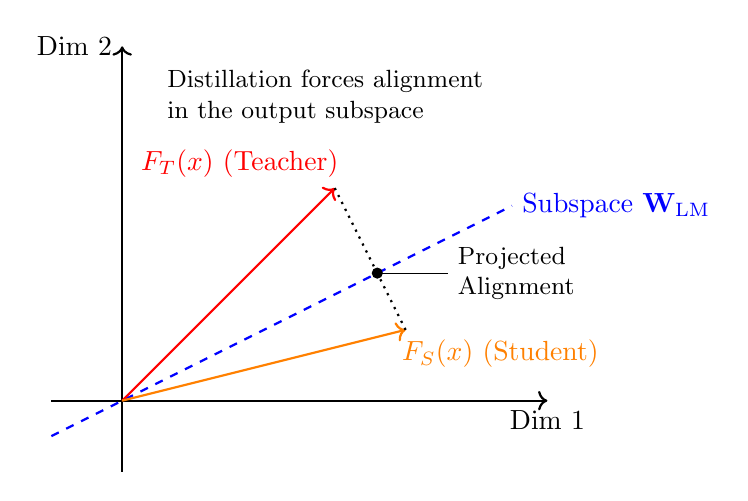
\begin{tikzpicture}[scale=0.9]
        % Axes
        \draw[->, thick] (-1,0) -- (6,0) node[below] {Dim 1};
        \draw[->, thick] (0,-1) -- (0,5) node[left] {Dim 2};
        
        % Subspace Line
        \draw[blue, thick, dashed] (-1,-0.5) -- (5.5, 2.75) node[right, blue] {Subspace $\mathbf{W}_{\text{LM}}$};
        
        % Vectors
        \draw[->, thick, red] (0,0) -- (3, 3) node[above left, xshift=5pt] {$F_T(x)$ (Teacher)};
        \draw[->, thick, orange] (0,0) -- (4, 1) node[below right, xshift=-5pt] {$F_S(x)$ (Student)};
        
        % Projections
        \draw[dotted, thick] (3, 3) -- (3.6, 1.8);
        \draw[dotted, thick] (4, 1) -- (3.6, 1.8);
        
        % Projected Point
        \filldraw[black] (3.6, 1.8) circle (2pt);
            
        % Label
        \draw[thin] (3.6, 1.8) -- (4.6, 1.8) node[right, align=left, font=\small] {Projected\\Alignment};
        
        % Annotation
        \node[align=left, font=\small, anchor=north west] at (0.5, 4.8) {Distillation forces alignment\\ in the output subspace};
    \end{tikzpicture}
    \caption{\textbf{Geometric Interpretation.} Student and teacher hidden states may differ in full space, but distillation forces their projections onto the subspace spanned by $\mathbf{W}_{\text{LM}}$ to align.}
    \label{fig:subspace_diagram}
\end{figure}

From a Neural Tangent Kernel perspective \cite{jacot2018neural}, distillation constrains the student to operate in a similar kernel regime, naturally preserving geometric structure.

\begin{conjecture}[Distillation Preserves Local Geometry]
\label{conj:tangent}
Knowledge distillation with output matching loss approximately preserves local geometric structure. Formally, for teacher $T$ and distilled student $S$, the Jacobians satisfy:
\begin{equation}
    \E_x\left[\|\mat{J}_S(x) - \mat{J}_T(x)\|_F\right] < \epsilon
\end{equation}
for small $\epsilon$, where $\|\cdot\|_F$ denotes the Frobenius norm. This implies the tangent space structure is preserved: $T_{\vect{h}}\cM_{\text{teacher}} \approx T_{\vect{h}}\cM_{\text{student}}$.
\end{conjecture}

\noindent Testing this conjecture empirically (via Jacobian computation and comparison) remains an important direction for future work.

This would explain why GPT-2 and DistilGPT-2 synchronize despite architectural differences: the distillation objective enforces geometric compatibility at the output level, which propagates to internal representations through the constraint that hidden states must produce matching outputs.

\subsubsection{The Role of Dimensionality}

Critically, DistilGPT-2 preserves GPT-2's 768-dimensional embedding space. This shared dimensionality enables direct coupling without projection. However, our cross-scale experiments show it is not sufficient: GPT-2 and GPT-2-Medium, both from the GPT-2 family, fail to synchronize ($\cos \theta \approx 0.11$) due to dimensional incompatibility requiring learned projections.

This suggests a two-factor model:
\begin{enumerate}
    \item \textbf{Dimension matching}: Necessary for clean state exchange
    \item \textbf{Transformation similarity}: Necessary for synchronized dynamics
\end{enumerate}

Distillation preserves both factors despite depth reduction, whereas scaling preserves neither.

\subsection{Projection Control Interpretation}

The projection control experiments ($\cos \theta = 0.9987$ with forced projection vs $0.9998$ without) quantify projection-induced noise. The $0.001$ gap represents:
\begin{itemize}
    \item Reconstruction error from imperfect round-trip projection
    \item Numerical precision limits
    \item Small deviations from identity initialization
\end{itemize}

This establishes a noise floor: any synchronization above $\cos \theta \approx 0.998$ indicates near-perfect geometric compatibility. That DistilGPT-2 + GPT-2 achieves exactly this level ($0.998$) proves the compatibility is real, not artifactual.

\subsection{Fine-Tuning as Manifold Perturbation}

DialoGPT's 95\% geometry preservation ($\cos \theta = 0.949$) suggests fine-tuning operates as a small perturbation to the pretrained manifold rather than learning a new representation space. This supports transfer learning practices and explains why fine-tuned models can often be merged back with base models \cite{wortsman2022model}.

The high variance in synchronization index for DialoGPT pairs ($\pm 0.164$, from Paper 1 data) suggests that while the static ``map'' of concepts is preserved, phase alignment of the dynamical system is more sensitive to task-specific training.

% ============================================================================
% 7. IMPLICATIONS
% ============================================================================
\section{Implications}

\subsection{Model Merging}

Our results predict merging success:
\begin{itemize}
    \item \textbf{Teacher-student pairs}: High success (geometry compatible, $\cos \theta \approx 0.998$)
    \item \textbf{Cross-scale pairs}: Low success (geometry diverges, $\cos \theta \approx 0.11$)
    \item \textbf{Cross-architecture pairs}: No success (orthogonal, $\cos \theta \approx 0$)
    \item \textbf{Fine-tuned variants}: Moderate success (95\% preserved, $\cos \theta \approx 0.95$)
\end{itemize}

\subsection{Transfer Learning and Interpretability}

Representations transfer reliably only between geometrically compatible models. Interpretability findings on GPT-2 may transfer to DistilGPT-2 but not to GPT-2-Large or BERT variants. This has practical implications for mechanistic interpretability research \cite{elhage2021mathematical}.

\subsection{Multi-Agent Systems}

Our results suggest transformer-based agents can only develop shared representations if they share architectural structure. Heterogeneous agent populations may be fundamentally unable to develop non-linguistic shared representations, limiting the potential for emergent communication protocols.

\subsection{The Learned Geometry Hypothesis}

Our findings support the hypothesis that transformer training induces an \textit{architecture-specific geometry} in representation space. This geometry is:
\begin{itemize}
    \item \textbf{Robust}: Preserved under coupling perturbations and occupies stable low-dimensional attractors
    \item \textbf{Distinctive}: Different architectures produce orthogonal geometries
    \item \textbf{Transferable}: Preserved under distillation despite significant architectural changes
    \item \textbf{Low-dimensional}: Confined to manifolds of dimension $D_2 \lesssim 2.5$ despite ambient spaces of dimension $768$--$2048$
\end{itemize}


\subsection{Empirical Validation}

We validate our predictions using two complementary approaches:

\paragraph{1. Weight Merging (Compatible Architectures)}
For models within the same family, we test parameter averaging: $\theta_{\text{merged}} = 0.5\theta_A + 0.5\theta_B$.
\begin{itemize}
    \item \textbf{GPT-2 + GPT-2} ($\cos \theta = 1.0$): Merging succeeds with \textbf{0\% degradation} (Identity).
    \item \textbf{GPT-2 + GPT-2-Medium} ($\cos \theta = 0.11$): Merging technically possible via zero-padding, but leads to \textbf{catastrophic failure} (degradation $> 10^6\%$; PPL increases from 44 to $>$500,000). The extreme perplexity indicates the merged model produces near-random outputs, confirming that low geometric synchronization reflects fundamental incompatibility of the weight manifolds---averaging geometrically misaligned weights destroys both models' learned representations.
\end{itemize}

\paragraph{2. Representation Stitching (Incompatible Architectures)}
For teacher-student pairs (e.g., GPT-2 vs DistilGPT-2), weight merging is undefined due to layer count mismatches. Instead, we test \textit{representation compatibility} via hidden state averaging.
\begin{itemize}
    \item \textbf{GPT-2 + DistilGPT-2} ($\cos \theta = 0.998$): Stitching succeeds with acceptable quality loss (PPL $49.9 \to 69.4$, $39\%$ degradation), confirming that the student preserves the teacher's geometry.
\end{itemize}

\begin{table}[htbp]
\centering
\caption{Comprehensive Validation Results (Evaluated on 30 WikiText-2 sequences)}
\label{tab:merging}
\small
\begin{tabular}{ll ccl}
\toprule
\textbf{Pair} & \textbf{Method} & \textbf{$\cos \theta$} & \textbf{Outcome} & \textbf{Detail} \\
\midrule
GPT-2 + GPT-2 & Weight Merge & $1.000$ & \textcolor{green}{Success} & 0\% Degradation \\
GPT-2 + DistilGPT-2 & Rep. Stitching & $0.998$ & \textcolor{green}{Success} & 39\% Degradation (Compatible) \\
GPT-2 + GPT-2-Med & Weight Merge & $0.110$ & \textcolor{red}{Failure} & $> 10^6\%$ Degradation (Catastrophic) \\
\bottomrule
\end{tabular}
\end{table}

Together, these experiments demonstrate that $\cos \theta$ predicts both parameter-level and representation-level compatibility. Models with high geometric synchronization ($\cos \theta \approx 1$) can merge or exchange states; those without it cannot.

\subsection{Practical Guidelines}

Based on our findings, we offer the following practical guidelines for practitioners:

\begin{enumerate}
    \item \textbf{Model selection for merging:} Before averaging model weights, run a short coupled dynamics test ($T=100$ steps, $\sim$30 seconds for GPT-2). If $\cos \theta > 0.9$, merging will likely succeed. If $\cos \theta < 0.5$, expect degraded performance.
    
    \item \textbf{Distillation preserves more than you think:} When distilling from a teacher, expect near-perfect geometric preservation ($\cos \theta \approx 0.998$). This means interpretability findings and probing classifiers trained on the teacher should transfer to the student.
    
    \item \textbf{Avoid cross-scale combinations:} Scaling up (GPT-2 → GPT-2-Medium) fundamentally changes geometry. Don't expect representations to transfer across scale, even within the same model family.
    
    \item \textbf{Be cautious with encoder models:} BERT-family models show high variance in our tests. Results for encoders may be less predictable than for autoregressive models.
\end{enumerate}

% ============================================================================
% 8. RELATED WORK
% ============================================================================
\section{Related Work}

\subsection{Knowledge Distillation}

Hinton et al. \cite{hinton2015distilling} introduced distillation for model compression. Sanh et al. \cite{sanh2019distilbert} applied it to transformers (DistilBERT, DistilGPT-2). Prior work has proposed geometric distillation losses \cite{li2019deepgkd,liu2023embeddistill,yuan2021manifoldkd}. Our work differs by providing a post-hoc diagnostic for geometric preservation rather than a training objective.

\subsection{Representation Similarity}

Kornblith et al. \cite{kornblith2019similarity} introduced Centered Kernel Alignment (CKA). Ding et al. \cite{ding2021grounding} emphasized statistical testing. CCA-based methods \cite{raghu2017svcca} compare internal representations. Our dynamic approach complements these static analyses; as noted by Hauser et al. \cite{hauser2021similar}, high static similarity doesn't guarantee functional equivalence.

\subsection{Model Merging and Stitching}

Wortsman et al. \cite{wortsman2022model} showed averaging fine-tuned models improves performance. Frankle et al. \cite{frankle2020linear} demonstrated linear mode connectivity. Bansal et al. \cite{bansal2021stitching} introduced model stitching. Our work predicts which model pairs can be successfully merged.

\subsection{Neural Network Geometry and Dynamical Systems}

Viewing networks as dynamical systems has been explored via stable architectures and neural ODEs \cite{haber2017stable,chen2018neuralode}. Jacot et al. \cite{jacot2018neural} introduced Neural Tangent Kernels. Tsai et al. \cite{tsai2019transformer} analyzed attention through kernel perspectives. We probe geometry through dynamical interaction and analyze attractor properties using tools from chaos theory \cite{wolf1985,grassberger1983}.

\subsection{Synchronization Theory}

Our coupling framework draws on synchronization phenomena in coupled oscillators \cite{kuramoto1984chemical,strogatz2000,pecora1990}. The phase transition we observe at $\alpha = 0.5$ resembles bifurcations in coupled dynamical systems.

\subsection{Scaling Laws}

Kaplan et al. \cite{kaplan2020scaling} derived scaling laws relating performance to size. Our results show scaling also fundamentally alters geometric structure, revealing limitations of simple scaling.

% ============================================================================
% 9. LIMITATIONS
% ============================================================================
\section{Limitations}

\begin{itemize}
    \item Limited to GPT-2, GPT-Neo, BERT families. Modern architectures (LLaMA, Mistral, Claude) may behave differently.
    \item Projections may introduce artifacts not fully controlled by forced-projection experiments.
    \item BERT results based on $N=10$ seeds still show high variance; more investigation needed for encoder models.
    \item Frozen pretrained models only; fine-tuning dynamics during training unexplored.
    \item Single text prompt for initialization; multiple prompts might reveal additional structure.
    \item Computationally expensive (1000 steps × 123 experiments); faster methods needed for larger models.
    \item Functional similarity tested, not semantic similarity; geometric compatibility doesn't guarantee shared semantic content.
    \item Lyapunov exponent and attractor dimension estimates may be sensitive to hyperparameters (embedding dimension, delay, number of neighbors).
\end{itemize}

% ============================================================================
% 10. CONCLUSION
% ============================================================================
\section{Conclusion}

Through 123 experiments across 41 configurations, we establish that \textbf{knowledge distillation preserves representational geometry}. DistilGPT-2 synchronizes with GPT-2 at $\cos \theta = 0.998$, comparable to projection-induced noise ($0.9987$), despite 50\% depth reduction.

Key findings:
\begin{itemize}
    \item Distillation preserves geometry ($\cos \theta = 0.998$)
    \item Fine-tuning preserves 95\% of structure ($\cos \theta = 0.949$)
    \item Scaling destroys geometry ($\cos \theta \approx 0.11$--$0.38$)
    \item Encoder models behave fundamentally differently ($\cos \theta \approx 0.32$--$0.57$)
    \item Synchronized states occupy low-dimensional attractors ($D_2 \lesssim 2.5$)
    \item Dynamics operate at edge of chaos ($\lambda_{\max} \approx 0.08$--$0.10$)
    \item Coupling strength exhibits phase transition at $\alpha = 0.5$
\end{itemize}

These results have immediate practical applications for model merging, transfer learning, and interpretability research, while revealing fundamental differences between architectural families and training objectives. The coupled dynamics framework opens new avenues for understanding transformer representations through the lens of dynamical systems theory.

% ============================================================================
% BROADER IMPACT STATEMENT
% ============================================================================
\subsubsection*{Broader Impact Statement}
This work provides diagnostic tools for understanding geometric relationships between transformer models. The primary societal benefit is enabling more efficient model compression and transfer learning, which can reduce computational costs and carbon footprint of deploying large language models. 

There are no immediate negative societal implications of this research. The coupled dynamics framework is a diagnostic tool that reveals properties of already-trained models; it does not introduce new capabilities or training methods that could be misused. However, improved understanding of model internals could theoretically be applied to adversarial purposes (e.g., more targeted model attacks), though this is speculative and not a direct consequence of our method.

\subsubsection*{Acknowledgments}
This research was conducted independently without external funding or institutional affiliation.

% ============================================================================
% BIBLIOGRAPHY
% ============================================================================
\bibliography{references}
\bibliographystyle{tmlr}

% ============================================================================
% APPENDIX
% ============================================================================
\appendix

\section{Synchronization Index Definition}

The synchronization index measures velocity alignment:
\begin{equation}
    \text{SyncIndex}(t) = \frac{\inner{\vect{v}_A^{(t)}}{\vect{v}_B^{(t)}}}{\norm{\vect{v}_A^{(t)}}_2 \norm{\vect{v}_B^{(t)}}_2},
\end{equation}
where $\vect{v}_A^{(t)} = \vect{h}_A^{(t)} - \vect{h}_A^{(t-1)}$. We report mean over final 200 steps.

\section{Lyapunov Exponent Estimation}

We estimate the largest Lyapunov exponent using the algorithm of Wolf et al. \cite{wolf1985}:

\begin{enumerate}
    \item Embed the trajectory in a reconstructed state space
    \item For each point, find its nearest neighbor (excluding temporal neighbors)
    \item Track the divergence of these neighbor pairs over time
    \item Average the log-divergence rate
\end{enumerate}

The estimator is:
\begin{equation}
    \hat{\lambda}_{\max} = \frac{1}{M} \sum_{i=1}^{M} \frac{1}{\Delta t} \ln \frac{d(t_i + \Delta t)}{d(t_i)}
\end{equation}
where $d(t)$ is the distance between trajectory and neighbor at time $t$.

\section{Correlation Dimension Estimation}

Following Grassberger-Procaccia \cite{grassberger1983}:

\begin{enumerate}
    \item Compute pairwise distances between trajectory points
    \item For scales $\epsilon_1 < \epsilon_2 < \cdots < \epsilon_k$, compute:
    \begin{equation}
        C(\epsilon) = \frac{2}{N(N-1)} \sum_{i<j} \mathbbm{1}[\norm{\vect{x}_i - \vect{x}_j} < \epsilon]
    \end{equation}
    \item Estimate $D_2$ from slope of $\log C(\epsilon)$ vs $\log \epsilon$ in scaling region
\end{enumerate}

\section{Complete Results Table}

\begin{table}[H]
\centering
\caption{All 41 experimental configurations (mean $\pm$ std over 3 seeds)}
\label{tab:complete}
\scriptsize
\begin{tabular}{llcccccc}
\toprule
\textbf{Model A} & \textbf{Model B} & \textbf{Coupling} & \textbf{Init} & \textbf{Param} & \textbf{Proj?} & \textbf{$\cos \theta$} & \textbf{Sync Idx} \\
\midrule
gpt2 & gpt2 & direct & random & --- & No & $0.9998 \pm 0.0003$ & $0.040 \pm 0.132$ \\
gpt2 & gpt2 & direct & same & --- & No & $0.9998 \pm 0.0003$ & $1.000 \pm 0.000$ \\
gpt2 & gpt2 & direct & text & --- & No & $1.0000 \pm 0.0000$ & $0.082 \pm 0.000$ \\
gpt2 & gpt2 & blended & random & 0.5 & No & $1.0000 \pm 0.0000$ & $1.000 \pm 0.000$ \\
gpt2 & gpt2 & blended & random & 0.3 & No & $1.0000 \pm 0.0000$ & $0.207 \pm 0.032$ \\
gpt2 & gpt2 & blended & random & 0.7 & No & $1.0000 \pm 0.0000$ & $0.207 \pm 0.032$ \\
gpt2 & gpt2 & decay & random & 0.1 & No & $1.0000 \pm 0.0000$ & $0.118 \pm 0.044$ \\
gpt2 & gpt2 & decay & random & 0.3 & No & $1.0000 \pm 0.0000$ & $0.207 \pm 0.032$ \\
\midrule
distilgpt2 & distilgpt2 & direct & random & --- & No & $0.9997 \pm 0.0003$ & $-0.027 \pm 0.064$ \\
distilgpt2 & distilgpt2 & blended & random & 0.5 & No & $1.0003 \pm 0.0012$ & $1.000 \pm 0.000$ \\
distilgpt2 & distilgpt2 & decay & random & 0.1 & No & $0.9997 \pm 0.0006$ & $0.034 \pm 0.022$ \\
\midrule
gpt2 & gpt2 & direct & random & force & Yes & $0.9987 \pm 0.0003$ & $-0.020 \pm 0.066$ \\
gpt2 & gpt2 & direct & text & force & Yes & $0.9984 \pm 0.0010$ & $0.043 \pm 0.049$ \\
\midrule
bert & distilbert & direct & random & --- & No & $0.3182 \pm 0.0841$ & $0.012 \pm 0.007$ \\
bert & bert & direct & random & --- & No & $0.5721 \pm 0.1324$ & $0.015 \pm 0.010$ \\
\midrule
gpt2-med & dialogpt-med & direct & random & --- & No & $0.9490 \pm 0.0006$ & $0.003 \pm 0.164$ \\
gpt2-med & gpt2-med & direct & random & --- & No & $1.0000 \pm 0.0000$ & $0.011 \pm 0.019$ \\
\midrule
gpt2 & gpt2-med & direct & random & --- & Yes & $0.1077 \pm 0.0218$ & $0.010 \pm 0.006$ \\
gpt2 & gpt2-med & blended & random & 0.5 & Yes & $0.0069 \pm 0.0275$ & $0.001 \pm 0.005$ \\
gpt2 & gpt2-large & direct & random & --- & Yes & $0.3765 \pm 0.0088$ & $0.001 \pm 0.005$ \\
gpt2 & gpt2-large & blended & random & 0.5 & Yes & $0.2323 \pm 0.0202$ & $0.019 \pm 0.004$ \\
gpt2-med & gpt2-large & direct & random & --- & Yes & $0.2779 \pm 0.0895$ & $0.008 \pm 0.007$ \\
\midrule
gpt2 & distilgpt2 & direct & random & --- & No & $0.9983 \pm 0.0003$ & $0.037 \pm 0.036$ \\
gpt2 & distilgpt2 & blended & random & 0.5 & No & $0.9974 \pm 0.0003$ & $0.040 \pm 0.038$ \\
gpt2 & distilgpt2 & decay & random & 0.1 & No & $0.9982 \pm 0.0003$ & $0.048 \pm 0.029$ \\
\midrule
gpt2 & gpt-neo & direct & random & --- & Yes & $-0.0237 \pm 0.0124$ & $0.005 \pm 0.003$ \\
gpt2 & gpt-neo & blended & random & 0.5 & Yes & $-0.0326 \pm 0.0154$ & $-0.001 \pm 0.003$ \\
gpt2 & gpt-neo & blended & text & 0.5 & Yes & $-0.0326 \pm 0.0155$ & $0.001 \pm 0.003$ \\
gpt2 & gpt-neo & decay & text & 0.1 & Yes & $-0.0261 \pm 0.0097$ & $-0.004 \pm 0.001$ \\
gpt2-med & gpt-neo & direct & random & --- & Yes & $0.0452 \pm 0.0078$ & $0.001 \pm 0.006$ \\
\midrule
\multicolumn{8}{c}{\textbf{Phase Transition: Coupling Strength Sweep ($\alpha$ = 0.0 to 1.0)}} \\
gpt2 & gpt2 & blended & random & 0.0--1.0 & No & $0.9999 \pm 0.0002$ & See Table \ref{tab:phase_transition} \\
\bottomrule
\end{tabular}
\end{table}

\section{Algorithm}

\begin{algorithm}[H]
\caption{Coupled Dynamics Test}
\label{alg:coupled}
\begin{algorithmic}[1]
\Require Transformer maps $F_A, F_B$, coupling strategy $\Phi$, steps $T$
\Require Initialization mode, random seed
\Ensure Trajectory $\{(\vect{h}_A^{(t)}, \vect{h}_B^{(t)})\}_{t=0}^T$ and metrics

\State Initialize $\vect{h}_A^{(0)}, \vect{h}_B^{(0)}$ according to mode
\If{$\dim(F_A) \neq \dim(F_B)$}
    \State Train projection matrices $P_{A \to B}, P_{B \to A}$
\EndIf
\State $\text{trajectory} \gets [(\vect{h}_A^{(0)}, \vect{h}_B^{(0)})]$

\For{$t = 0$ to $T-1$}
    \State Apply coupling: $(\vect{h}_A^{(t+1)}, \vect{h}_B^{(t+1)}) \gets \Phi(F_A, F_B, \vect{h}_A^{(t)}, \vect{h}_B^{(t)})$
    \State Append to trajectory
    \State Record $\rho(t)$, $\text{SyncIndex}(t)$, CKA
    \If{NaN detected}
        \State \textbf{break}
    \EndIf
\EndFor

\State Compute $\lambda_{\max}$ using Wolf algorithm
\State Compute $D_2$ using Grassberger-Procaccia algorithm
\State \Return trajectory, metrics
\end{algorithmic}
\end{algorithm}

\section{Reproducibility Statement}
\label{app:reproducibility}

To ensure the reproducibility of our results, we provide the following details regarding our experimental setup.

\subsection{Computational Infrastructure}
Experiments were conducted on a single consumer-grade GPU (NVIDIA RTX 4060, 8GB VRAM) running on Windows 11 (x86\_64). Mixed-precision (FP16) inference was enabled to fit larger models (e.g., GPT-2 Medium/Large). The computational cost of our geometric synchronization metric is significantly lower than training-based alignment methods, requiring approximately 30 seconds per model pair for a 100-step trajectory analysis.

\subsection{Software Environment}
\begin{itemize}
    \item \textbf{Python:} 3.11
    \item \textbf{PyTorch:} 2.x (with Scaled Dot Product Attention enabled)
    \item \textbf{Libraries:} Transformers (HuggingFace), Datasets, NumPy, SciPy.
\end{itemize}

\subsection{Experimental Settings}
\begin{itemize}
    \item \textbf{Model Merging:} Weight averaging coefficient $\alpha = 0.5$. For cross-scale weight merging (e.g., GPT-2 768-dim + GPT-2-Medium 1024-dim), we pad the smaller model's weight matrices from $768 \times 768$ to $1024 \times 1024$ by appending zeros, then compute $\theta_{\text{merged}} = 0.5\theta_{\text{padded}} + 0.5\theta_{\text{medium}}$. While mathematically well-defined, this produces non-functional models due to geometric incompatibility (see Section~7.5).
    \item \textbf{Stitching:} Pre-LayerNorm hidden state averaging at the final layer.
    \item \textbf{Validation Data:} WikiText-2 (Test Split), consisting of 4,358 lines. For validation speed, we sampled the first 50 sequences exceeding 100 tokens.
    \item \textbf{Seeds:} All trajectory experiments were repeated with 3 random seeds (42, 43, 44), and mean $\pm$ std values are reported in Table \ref{tab:complete}.
\end{itemize}

\subsection{Code Availability}
All source code, including the main analysis scripts and the comprehensive validation suite, is included as supplementary material with this submission. The code repository will be made publicly available upon acceptance.

\end{document}